\begin{answer}

Observe the plot of dataset 1, on x1 axis the data point
on roughly follows Gaussian, but on x2 axis the point density 
looks like a exponential distribution which has a big head
and small a tail. It can also be seen as $\chi^2$ distribution,
which can be seen as sum square of k Gaussians,  which leads to the 
first two transformation. 

The third log transformation also looking good.

    \begin{figure}[h]
        \centering
        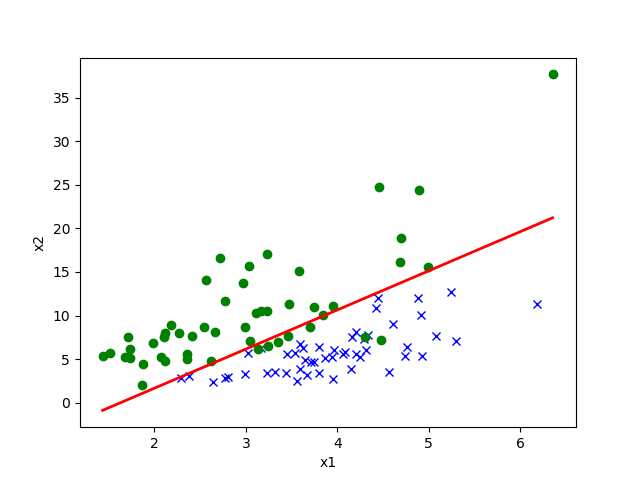
\includegraphics[width=0.6\textwidth]{p01e_pred_1_txt_gda_valid_2}
        \caption{ x2 = sqrt(x2) on validation set}
    \end{figure}
    
    \begin{figure}[h]
        \centering
        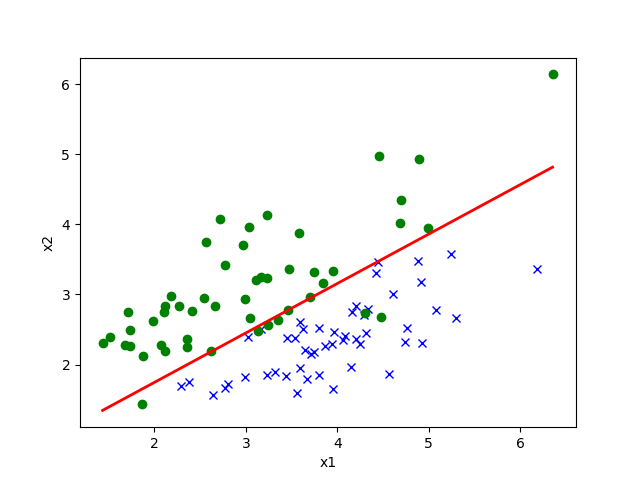
\includegraphics[width=0.6\textwidth]{p01e_pred_1_txt_gda_valid_4}
        \caption{ x2 = $(x2)^{\frac{1}{4}}$ on validation set }
    \end{figure}
    
    \begin{figure}[h]
        \centering
        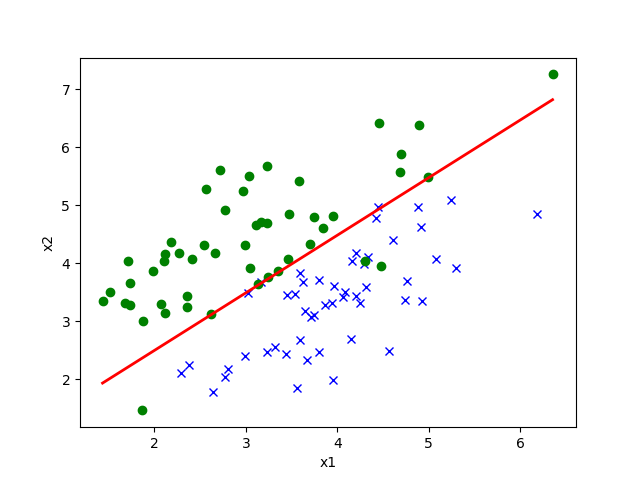
\includegraphics[width=0.6\textwidth]{p01e_pred_1_txt_gda_valid_log}
        \caption{ x2 = log(x2) validation set }
    \end{figure}

\end{answer}
